En este sprint denominado el \textit{"Sprint 0"}, se definieron aspectos fundamentales para el éxito del proyecto, con el objetivo de preparar al equipo y el entorno para los sprints de desarrollo regulares. 

\begin{itemize}
    \item Se realizó un análisis exhaustivo del stack tecnológico que se usará para el desarrollo, tanto del lado del frontend como del backend, abordando cada uno de los dos backends y los cuatro componentes diferentes del sistema, los cuales son:
    \begin{itemize}
        \item Gestión de perfiles de usuarios del sistema (Admin y pruebas de funcionalidad de usuarios logueados).
        \item Desarrollo de módulo que implemente funciones del tipo red social para los usuarios del sistema.
        \item Implementación de estrategia(s) de mediación o facilitación del consenso (sistema como mediador para el grupo de investigadores).
        \item Desarrollo del módulo de Analítica: Dashboards y estadísticas para la toma de decisiones.
    \end{itemize}
    El propósito de este análisis es garantizar que tanto el frontend como el backend utilicen las tecnologías más apropiadas para satisfacer los requisitos técnicos y de negocio, y para así asegurar una integración efectiva y eficiente entre todas las partes del sistema.
    

    Así se tomaron las siguientes decisiones:
    \begin{enumerate}
        \item Para la integración del sistema  en el lado del frontend se optó por utilizar Angular como framework de desarrollo, debido a que se puede reutilizar componentes de el sistema ResNet \cite{RESNET}. 
        \item Para el lado del backend se propuso utilizar Django como framework. Con Django, se espera aprovechar su robustez, seguridad y su capacidad para desarrollar rápidamente aplicaciones web escalables y de alto rendimiento. Además, Django ofrece una amplia gama de características integradas, como autenticación de usuarios, administración de bases de datos, y un ORM\footnote{ORM (Object-Relational Mapping) es una herramienta que facilita la comunicación y traducción de datos entre bases de datos relacionales y objetos en programación orientada a objetos.} potente, lo que lo hace una elección sólida para el desarrollo del backend del sistema. 
        \item Para mantener las mismas dependencias de desarrollo y simplificar la gestión del entorno, se utilizará Docker \cite{DOCKER}. Esto permite encapsular aplicaciones y sus dependencias en contenedores, asegurando consistencia entre entornos.
        \item Además, Docker Compose se empleará para orquestar el servidor backend y la base de datos, facilitando la configuración y gestión del entorno, y simplificando el despliegue del sistema en diferentes entornos.
        \item La elección de Neo4j se basa en la decisión de no alterar el modelo de datos actual. Dado que Neo4j está especialmente diseñado para modelos de datos conectados y relacionales, su adopción evita la necesidad de reestructurar el modelo existente, ahorrando tiempo y recursos mientras garantiza la continuidad del desarrollo del sistema.
        \item El control de versiones se hará mediante Git y para alojar dichas versiones se utilizará GitHub. Mediante una organización en donde se alojará el código fuente de los 4 componentes.
        \item Para la gestión del proyecto, se utilizó SCRUM en conjunto con Azure DevOps \cite{AZURE-DEVOPS}. SCRUM proporciona un marco ágil para la planificación y ejecución de proyectos, mientras que Azure DevOps \cite{AZURE-DEVOPS} ofrece herramientas integradas para facilitar todas las etapas del ciclo de vida del desarrollo de software. Esta combinación garantiza una gestión eficiente y colaborativa del proyecto, mejorando la transparencia y la entrega oportuna de resultados.
        En la Figura \ref{fig:azure-devops-project} se muestra el proyecto en Azure DevOps.
        \begin{figure}[H]
            \centering
            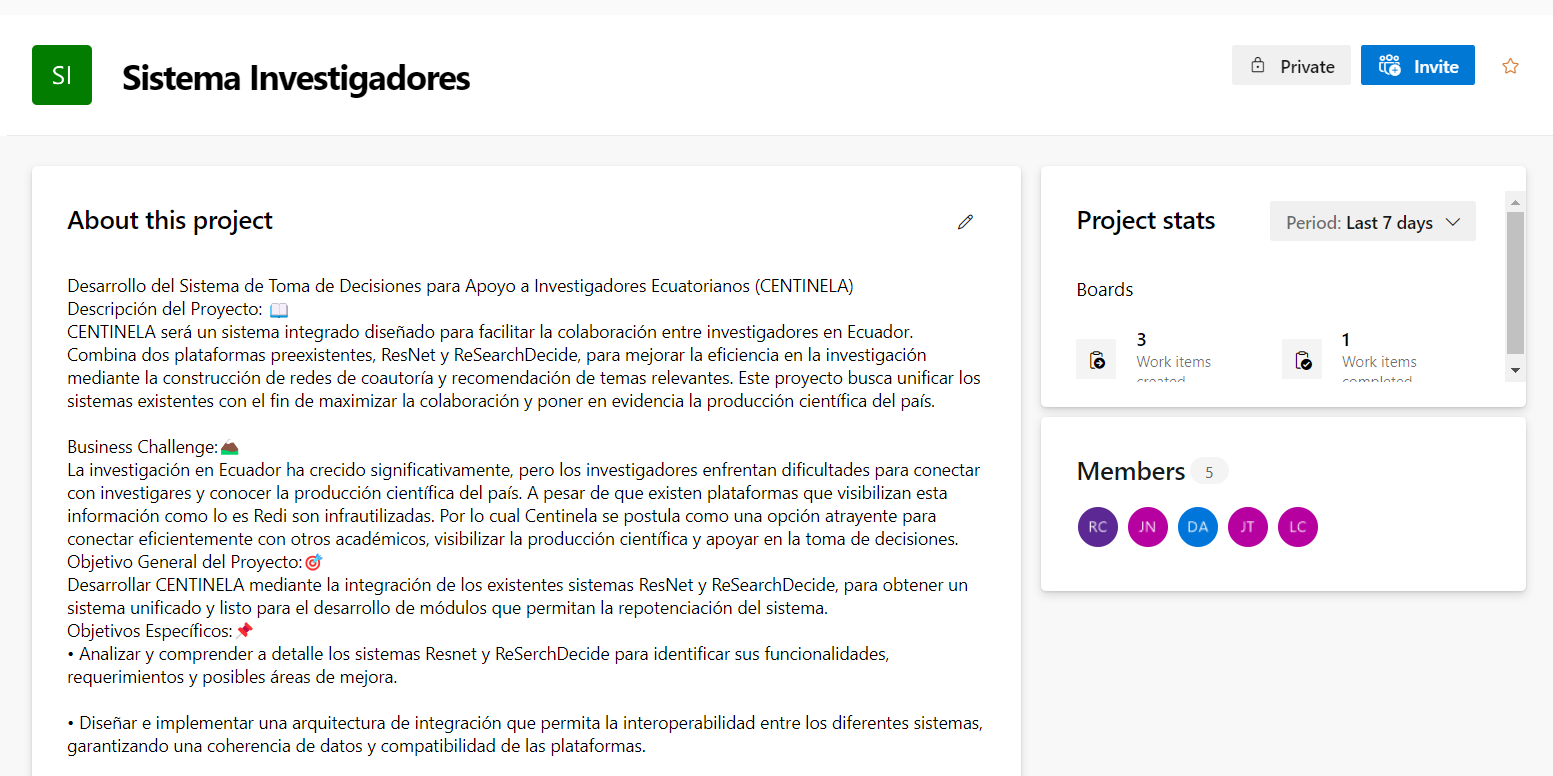
\includegraphics[width=0.5\linewidth]{02Figures//02Chapter//Sprints//Sprint-0/azure-devops-project.png}
            \caption{Proyecto en Azure DevOps}
            \label{fig:azure-devops-project}
        \end{figure}
        \item Se optó por Visual Studio Code como editor de código para el frontend y PyCharm como IDE de desarrollo especializado para el backend. Esta elección proporcionó un entorno flexible y eficaz para la colaboración en el proyecto.
    \end{enumerate}

    \item Se establecieron horarios para las reuniones diarias, las cuales se llevarán a cabo los días lunes, martes, miércoles y jueves en el horario de 14:00 a 16:00 en un espacio proporcionado por la directora del proyecto, Lorena Recalde, en el edificio de Sistemas. Durante este intervalo, se realizaron los daily meetings y se llevó a cabo el trabajo en equipo.

    \item Se  decidió adoptar el inglés como el idioma oficial para la codificación, los commits y toda la documentación técnica dentro de nuestro equipo. Esta medida busca estandarizar nuestras prácticas con los estándares internacionales, facilitar la colaboración con otros equipos y mejorar la accesibilidad a recursos técnicos de alta calidad.

    \item Se decidió utilizar Arquitectura Hexagonal \cite{ARQUITECTURA-HEXAGONAL} como patrón de arquitectura, definiendo así una estructura de carpetas y respetando los principios de esta arquitectura. Cabe destacar que no se ha implementado arquitectura hexagonal en su totalidad, ya que se optó por una adaptación de la misma, obteniendo así una arquitectura de dos capas.
    \begin{itemize}
        \item \textbf{Backend}: Para el backend, en cuanto a  la estructura de carpetas, se definió que por cada módulo en general se tendrá las tres  capas de arquitectura como son infraestructura, aplicación y dominio como se muestra en la Figura \ref{fig:hexagonal-architecture-example-backend}.

        \begin{figure}[H]
            \centering
            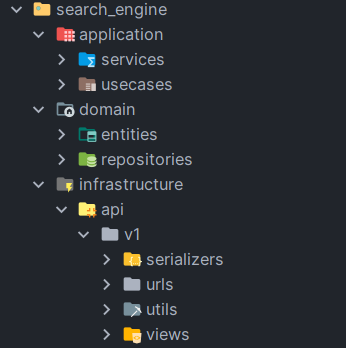
\includegraphics{02Figures/02Chapter/Sprints/Sprint-0/hexagonal-architecture-example.png}
            \caption{Arquitectura Hexagonal aplicada en el modulo del motor de búsqueda}
            \label{fig:hexagonal-architecture-example-backend}
        \end{figure}
        \item \textbf{Frontend}: Basándonos en el concepto de puertos y adaptadores, en el frontend también hemos optado por  implementar la Arquitectura Hexagonal \cite{ARQUITECTURA-HEXAGONAL} como patrón de arquitectura, con algunas adaptaciones específicas para este contexto. Dado que el frontend se enfoca en la parte gráfica, el adaptador se denominará "presentación", donde se gestionará toda la interfaz gráfica. Esta capa de presentación será el punto de entrada hacia el núcleo (core) de la aplicación frontend, facilitando así una separación clara entre la lógica de negocio y la interfaz de usuario, y promoviendo una estructura modular y fácilmente mantenible (Figura \ref{fig:hexagonal-architecture-example-frontend}.)
        \begin{figure}[H]
            \centering
            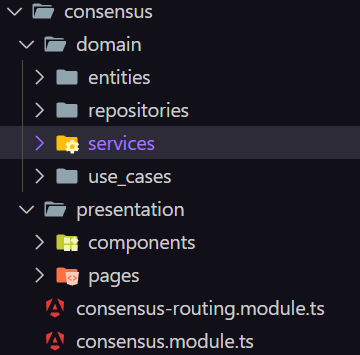
\includegraphics{02Figures/02Chapter/Sprints/Sprint-0/hexagonal-architecture-example-frontend.png}
            \caption{Arquitectura hexagonal aplicada al modulo de consenso}
            \label{fig:hexagonal-architecture-example-frontend}
        \end{figure}
    \end{itemize}
\end{itemize}